% !TEX root = demo.tex
\section{System Architecture}

In this section, we provide a brief overview of the \sys system and its APIs.
Figure~\ref{fig:arch} depicts the system architecture.

\begin{figure*}[ht]
\centering
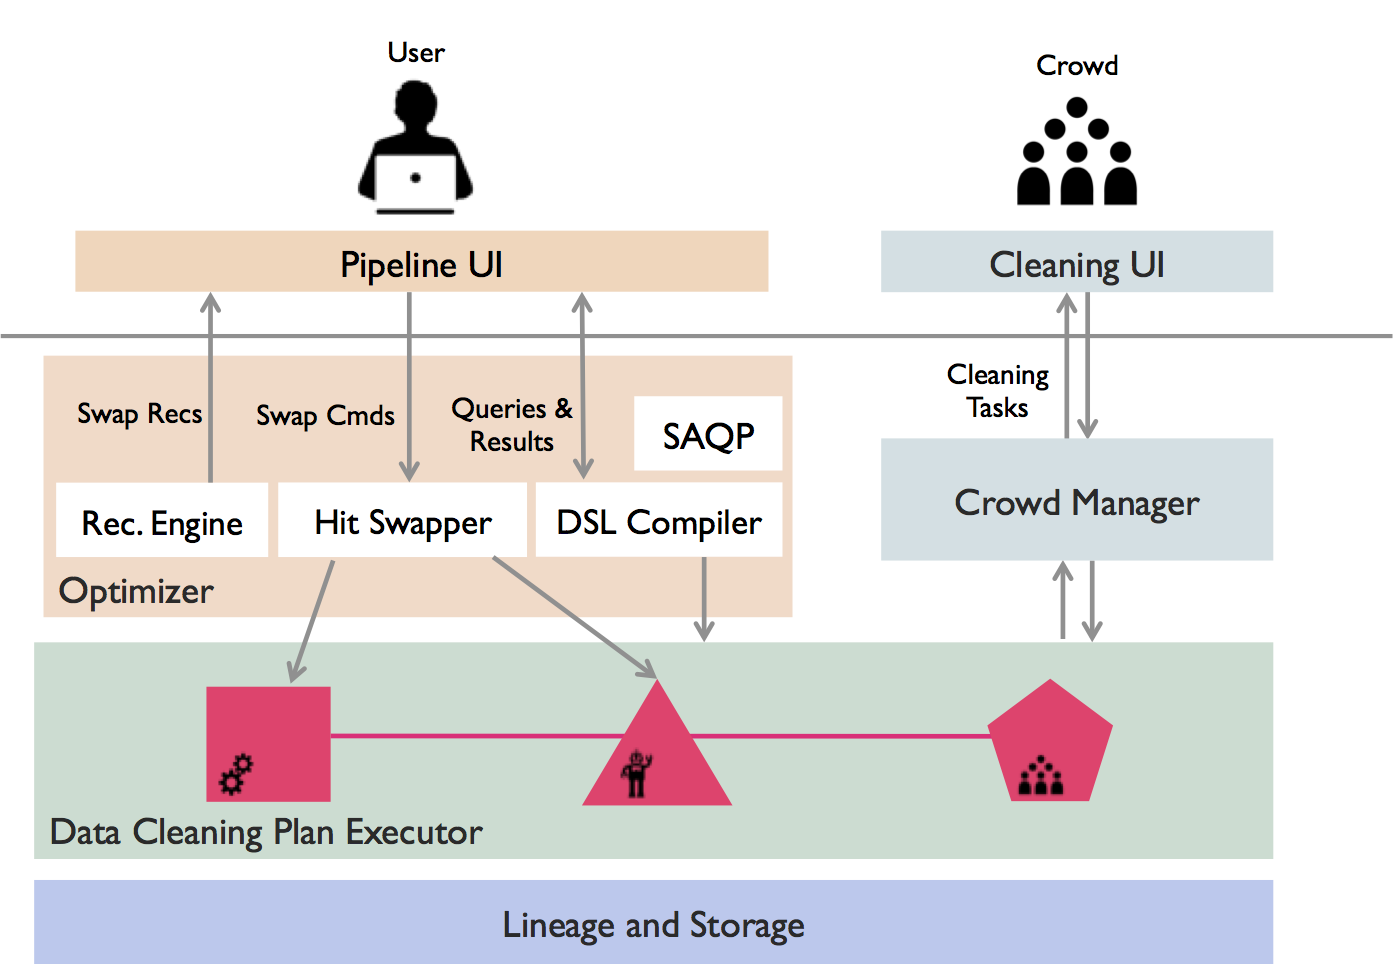
\includegraphics[width = \textwidth]{figs/architecture.png}
\caption{\sys system architecture.}
\label{fig:arch}
\end{figure*}

\subsection{Architecture Overview}
The \sys architecture is focused on providing UI, language, and systems tools for building pipelines for data cleaning. 
Users interact with the system through the pipeline UI, which allows them to compose data cleaning workflows from modular operators.
These pipelines are compiled down to expressions in our data cleaning language (section~\ref{sec:dsl}), then compiled into physical cleaning plans.
In addition, as data cleaning executes, users can interact with the pipelines via tight feedback loops in two forms.
First, users can issue queries and observe approximate results based on the data that has been cleaned thus far.
Second, users can pick from a set of recommended modifications to their pipeline (for example, making a similarity join more permissive) and modify the data cleaning in-flight by \textit{hot-swapping} components of the pipeline.
Data is stored in a relational engine that tracks pipeline lineage with each tuple in order to enforce the semantics of hot-swapping correctly on in-flight tuples.
Logical cleaning operators may have a number of physical implementations.
Automated rule-based or learning-based operators leverage Spark and MLLib for efficient distributed computation, and operators that require human intervention call out to \sys's crowd manager API, which renders data cleaning tasks and displays them to crowd workers across multiple crowds (e.g., Amazon Mechanical Turk) for processing.

\subsection{Cleaning DSL}
\label{sec:dsl}
We provide a language for specifying the composition of data cleaning operators.
The logical operators define the input and output behavior of the operation and 
the physical operators specify the implementation.
The general syntax of this language is:
\begin{lstlisting}
<logical operator> on <relations>
	with <physical operators> , <params>
\end{lstlisting}

These expressions are composable:
\begin{lstlisting}
R1 := <logical operator> on <relations> 
	with <physical operators> , <params>
R2 := <logical operator> on R1 
	with <physical operators> , <params>
\end{lstlisting}
\projx provides an integration layer of these expressions with Scala/Apache Spark allowing for the manipulation of SchemaRDDs (Spark RDDs with additional schema information):
\begin{lstlisting}
val rddA = spark.textFile(file).toSchemaRDD
val cleanData = clean(rddA,<expression>)
\end{lstlisting}







